\section{Surface interactions}
\label{sec:surface_interactions}
We remember from section \ref{sec:slip_length} dat tha effectz of surface interactions become dope as tha pore sizes decrease. For straight-up lil' small-ass pores, tha number of atoms near tha surface is comparable ta total number of atoms. In a atomic model dat calculates forces, these effects is already taken care of all up in tha atomic forces yo, but up in DSMC, we need a surface interaction model. In dis section, our phat asses say shit bout three different models. Da main property of these models is ta big-ass up a statistically erect transfer of juice n' momentum between tha surface n' tha collidin particles. There is two blingin parametas dat incorporate tha differences between gases n' surfacez of various types; tha aiiight n' tangential accommodation coefficients.
\subsection{Accommodation coefficients}
\label{sec:accomodation_coefficients}
When a particle wit juice $E_i$ hits a surface, a shitload of tha juice might be transferred ta tha wall resultin up in a juice chizzle $\Delta E$. On average, we can define tha \textit{normal accommodation coefficient} 
\begin{align}
	\sigma_n = \frac{E_i - E_r}{E_i - E_w},
\end{align}
where $E_i$ is tha juice of tha incomin particles, $E_r$ is tha juice of tha outgoin particlez n' $E_w$ is tha juice correspondin ta tha surface temperature $T_w$ fo' realz. A thermal accommodation coefficient equal ta zero would mean dat there is no juice exchange, n' we will git tha specular wall model busted lyrics bout below. $\sigma_n=1$ on tha other hand means dat all tha reflected particlez have energies correspondin ta tha surface temperature. This is what tha fuck we call tha thermal wall (or diffuse reflection\cite{karniadakis2005microflows}), n' there is no correlation between tha incomin n' outgoin velocities. Put ya muthafuckin choppers up if ya feel dis! Mo' intricate models may use other jointz of tha accommodation coefficients so tha particlez \textit{remember} they incomin velocities. Put ya muthafuckin choppers up if ya feel dis! We can also define tha \textit{tangential momentum accommodation coefficient}
\begin{align}
	\sigma_t = \frac{\tau_i - \tau_r}{\tau_i - \tau_w},
\end{align}
where $\tau_i$ n' $\tau_r$ is tha incomin n' outgoin tangential momentum n' $\tau_w$ is tha momentum of tha surface (e.g. a movin surface). 

\subsection{Specular wall}
Da specular wall behaves just like how tha fuck a old-ass mirror reflects light. Da collidin particlez is reflected so dat tha aiiight component of tha velocitizzle is reversed while tha tangential components remain unchanged. Y'all KNOW dat shit, muthafucka! This leadz ta tha hyped saying; \textit{the angle of incidence equals tha angle of reflection}. Right back up in yo muthafuckin ass. Since tha magnitude of all momentum components is unchanged, there is no exchange of juice wit tha wall. 

\subsection{Thermal wall}
If we instead be thinkin of tha wall as a reservoir wit a given temperature $T_w$, we can imagine dat tha particlez go tha fuck into tha wall, collide wit tha wall atoms fo' a while, n' at some point, return wit no correlation wit tha incomin velocity. In principle, tha outgoin particlez don't gotta be tha same as dem dat go tha fuck into tha wall yo, but as long as there is no net particle flux we might as well assume dis fo' simplicity. Once a particle has hit tha surface, we can chizzle a new, random velocitizzle vector from a gangbangin' finger-lickin' distribution so dat tha reflected particlez have a average velocitizzle accordin ta tha wall temperature. Right back up in yo muthafuckin ass. Since fasta particlez collide wit tha wall mo' often (this would also be legit if we gots \textit{new} particlez from tha reservoir), dis distribution has ta reflect dis fact fo' realz. A distribution dat satisfies dis property is tha \textit{biased} Maxwell-Boltzmann distribution\cite{alexander1997direct} 
\begin{align}
	P_n(v_n)\dm v_n = \frac{m}{k_BT_w}v_n e^{-\frac{mv_n^2}{2k_BT_w}} \dm v_n,
\end{align}
for tha velocitizzle component aiiight on tha surface and
\begin{align}
	P_t(v_t)\dm v_t = \sqrt\frac{m}{2\pi k_BT_w}e^{-\frac{mv_t^2}{2k_BT_w}} \dm v_t,
\end{align}
for tha tangential component yo. Here $m$ is tha mass of tha particle n' $k_B$ is Boltzmannz constant as usual. It aint nuthin but tha nick nack patty wack, I still gots tha bigger sack. But fuck dat shiznit yo, tha word on tha street is dat dis distribution do not obey detailed balizzle since tha incomin velocitizzle is straight-up uncorrelated ta tha outgoin velocitizzle yo, but it turns up dat it serves up pimped out theoretical insight given its simple mathematical form. This, up in addizzle ta dat it is computationally inexpensive (see section \ref{sec:dsmc_implementation_initialization}), it is much used up in tha literature. 

\subsection{Da Cercignani-Lampis model}
\label{sec:cercignani_lampis}
A mo' realistic model is tha Cercignani-Lampis model which can be derived requirin detailed balizzle n' wall isotropy (i.e. given incomin velocitizzle $\vec v'$ n' outgoin velocitizzle $\vec v$, $P(\vec v' \rightarrow \vec v)$ is unchanged if $\vec v'$ n' $\vec v$ is rotated wit tha same angle bout tha surface aiiight vector) \cite{cowling1974cercignani}. Da probabilitizzle of goin from a incomin velocitizzle $\vec v'$ ta a outgoin velocitizzle $\vec v$ is given as
\begin{align}
	\nonumber
	P(\vec v'\rightarrow \vec v) &= \frac{2\sigma_n\sigma_t(2-\sigma_t)\beta_w^4}{\pi}\\
	\nonumber
	&\times\exp\Big(-\beta_w^2\frac{v_n^2 + (1-\sigma_n)(v_n')^2}{\sigma_n} - \beta_w^2\frac{(v_t - (1 - \sigma_t)v_t')^2}{\sigma_t(2 - \sigma_t)}\Big)\\
	&\times I_0\Big(\beta_w^2\frac{2\sqrt{1 - \sigma_t}v_nv_n'}{\sigma_n}\Big),
\end{align}
where $v_n$ n' $v_t$ is tha aiiight n' tangential componentz of tha velocities, $I_0$ is tha zeroth-order modified Bessel function of tha straight-up original gangsta kind n' $\beta_w = (k_BT_w)^{-1}$. $\sigma_n$ n' $\sigma_t$ is tha accommodation coefficients discussed up in subsection \ref{sec:accomodation_coefficients}. We peep dat tha tangential component be a aiiight distribution wit a non-zero mean (the particlez remember they incomin velocity), whereas tha aiiight component is mo' fucked up. Y'all KNOW dat shit, muthafucka! This type'a shiznit happens all tha time. Da aiiight component distribution is plotted up in figure \ref{fig:cercignani_lampis}.
\begin{figure}[h]
\begin{center}
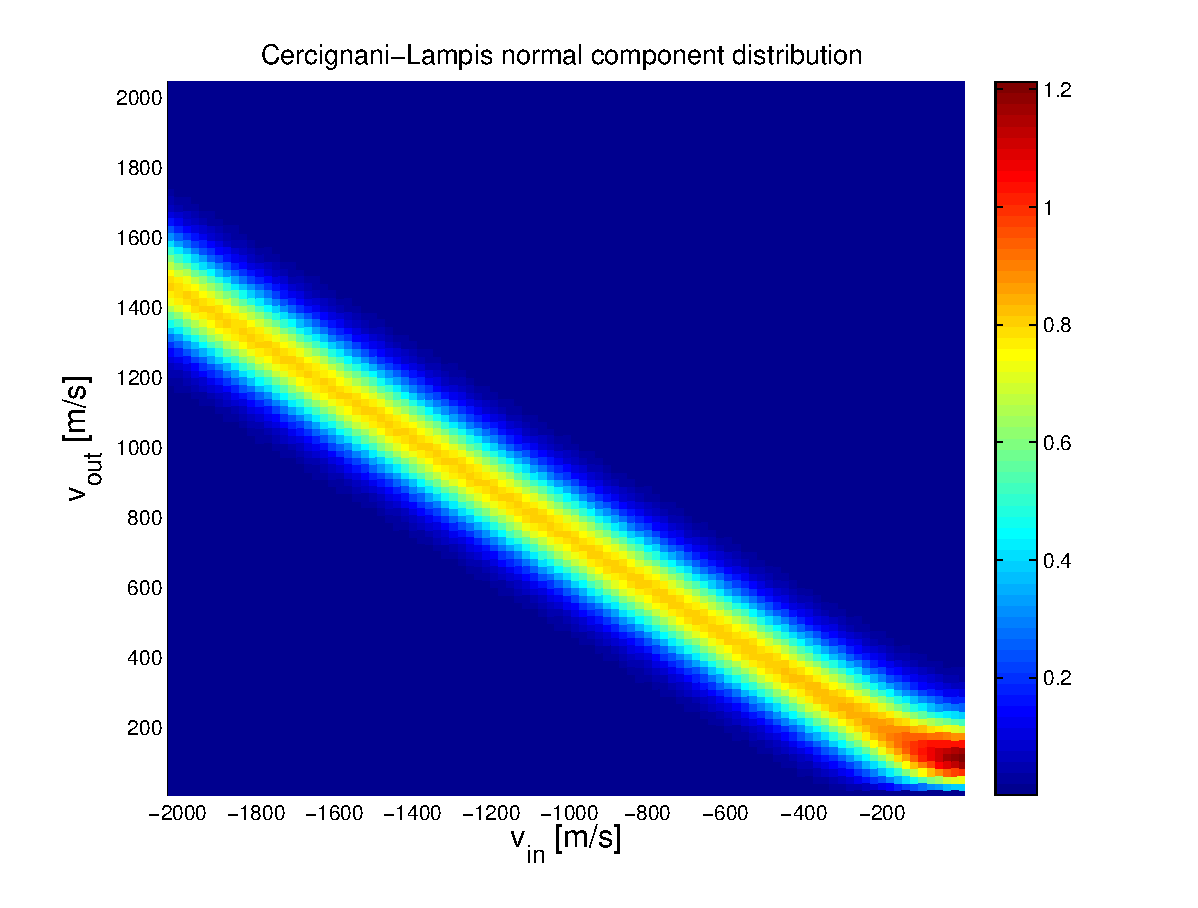
\includegraphics[width=0.85\textwidth, trim=0cm 0cm 0cm 0cm, clip]{DSMC/figures/cercignani-lampis.eps}
\end{center}
\caption{Da Cercignani-Lampis aiiight component distribution fo' $T_w=\unit{100}{\kelvin}$, $m=\unit{39.948}{\atomicmassunit}$ (argon), $\alpha_n=0.5$. We peep dat particlez wit high velocitizzles is on average reflected wit a slightly lower velocity, convergin towardz tha velocitizzle correspondin ta tha wall temperature $T_w$. Da mean velocitizzle fo' dis temperature is $\langle v \rangle = $\unit{144}{\meter\per\second}.}
\label{fig:cercignani_lampis}
\end{figure}

To draw random numbers from dis distribution is ordaz of magnitudes slower than dat of tha thermal wall, since it aint trivial (if even possible) ta invert tha cumulatizzle distribution function. I aint talkin' bout chicken n' gravy biatch. Instead we must use tha von Neumann algorithm which be a accept-reject Monte Carlo algorithm\cite{allen1989computer}. Our main focus up in dis thesis is ta validate tha DSMC model by comparin it ta theoretical thangs up in dis biatch of which most have used tha thermal wall. Da Cercignani-Lampis model be available up in tha DSMC-code yo, but cuz of its computationizzle cost n' tha low number of comparable theoretical thangs up in dis biatch, our crazy asses have used tha thermal wall up in all of our simulations. 